\documentclass[a4paper,12pt]{Latex/Classes/PhDthesisPSnPDF}
\usepackage[utf8]{inputenc}
\usepackage{amsthm}
\usepackage{graphicx}

% \usepackage[spanish]{babel}
\input{body/preamble/preamble.Rnw}
% This file contains macros that can be called up from connected TeX files
% It helps to summarise repeated code, e.g. figure insertion (see below).

%%%%%%%%%%%%%%%%%%%%%%%%%%%%%%%%%%%%%%%%%%%%%%
%            Colores de la UNAM              %
%%%%%%%%%%%%%%%%%%%%%%%%%%%%%%%%%%%%%%%%%%%%%%
%Azul Pantone 541  -->(0,63,119) RGB
\definecolor{Azul}{RGB}{128,0,0}

%Oro Pantone 460  -->(234,221,150) RGB
\definecolor{Oro}{RGB}{234,221,150}


%%%%%%%%%%%%%%%%%%%%%%%%%%%%%%%%%%%%%%%%%%%%%%
%            Comandos para líneas            %
%%%%%%%%%%%%%%%%%%%%%%%%%%%%%%%%%%%%%%%%%%%%%%
%Se define un comando \colorvrule para hacer líneas verticales de color con 3 argumentos: color, ancho, alto
\newcommand{\colorvrule}[3]{
\begingroup\color{#1}\vrule width#2 height#3
\endgroup}

%Se define un comando \colorhrule para hacer líneas horizontales de color con 2 argumentos: color, ancho
\newcommand{\colorhrule}[2]{
\begingroup\color{#1}\hrule height#2
\endgroup}

%%%%%%%%%%%%%%%%%%%%%%%%%%%%%%%%%%%%%%%%%%%%%%
%          Comando para derivadas            %
%%%%%%%%%%%%%%%%%%%%%%%%%%%%%%%%%%%%%%%%%%%%%%
\newcommand{\derivada}[3][]{\ensuremath{\dfrac{\mbox{d}^{#1}#2}{\mbox{d}#3^{#1}}}} 
%primer argumento(opcional): orden de la derivada
%segundo argumento: función a derivar
%tercer argumento: variable respecto a la que se deriva


%%%%%%%%%%%%%%%%%%%%%%%%%%%%%%%%%%%%%%%%%%%%%%
%       Comando para la exponencial          %
%%%%%%%%%%%%%%%%%%%%%%%%%%%%%%%%%%%%%%%%%%%%%%
\newcommand{\e}[1][]{\ensuremath{\mbox{e}^{#1}}}
%primer argumento(opcional): exponente de la exponencial




% insert a centered figure with caption and description
% parameters 1:filename, 2:title, 3:description and label
\newcommand{\figuremacro}[3]{
	\begin{figure}[htbp]
		\centering
		\includegraphics[width=1\textwidth]{#1}
		\caption[#2]{\textbf{#2} - #3}
		\label{condicion}
	\end{figure}
}

% insert a centered figure with caption and description AND WIDTH
% parameters 1:filename, 2:title, 3:description and label, 4: textwidth
% textwidth 1 means as text, 0.5 means half the width of the text
\newcommand{\figuremacroW}[4]{
	\begin{figure}[htbp]
		\centering
		\includegraphics[width=#4\textwidth]{#1}
		\caption[#2]{\textbf{#2} - #3}
		\label{#1}
	\end{figure}
}

% inserts a figure with wrapped around text; only suitable for NARROW figs
% o is for outside on a double paged document; others: l, r, i(inside)
% text and figure will each be half of the document width
% note: long captions often crash with adjacent content; take care
% in general: above 2 macro produce more reliable layout
\newcommand{\figuremacroN}[3]{
	\begin{wrapfigure}{o}{0.5\textwidth}
		\centering
		\includegraphics[width=0.48\textwidth]{#1}
		\caption[#2]{{\small\textbf{#2} - #3}}
		\label{#1}
	\end{wrapfigure}
}

% predefined commands by Harish
\newcommand{\PdfPsText}[2]{
  \ifpdf
     #1
  \else
     #2
  \fi
}

\newcommand{\IncludeGraphicsH}[3]{
  \PdfPsText{\includegraphics[height=#2]{#1}}{\includegraphics[bb = #3, height=#2]{#1}}
}

\newcommand{\IncludeGraphicsW}[3]{
  \PdfPsText{\includegraphics[width=#2]{#1}}{\includegraphics[bb = #3, width=#2]{#1}}
}

\newcommand{\InsertFig}[3]{
  \begin{figure}[!htbp]
    \begin{center}
      \leavevmode
      #1
      \caption{#2}
      \label{#3}
    \end{center}
  \end{figure}
}







%%% Local Variables:
%%% mode: latex
%%% TeX-master: "~/Documents/LaTeX/CUEDThesisPSnPDF/thesis"
%%% End:
 
\newtheorem{teorema}{Teorema}
\newtheorem{definicion}{Definición}
% \showboxdepth=5
% \showboxbreadth=5
%%%%%%%%%%%%%%%%%%%%%%%%%%%%%%%%%%%%%%%%%%%%%%%%%%%%%%%%%%%%%%%%%%%%%%%%%%%%%%%%
%                                   DATOS                                      %
%%%%%%%%%%%%%%%%%%%%%%%%%%%%%%%%%%%%%%%%%%%%%%%%%%%%%%%%%%%%%%%%%%%%%%%%%%%%%%%%
\title{Evaluación de la Efectividad del Método GARCH-EVT-COPULAS para el cálculo del VaR como Medida de Riesgo en Mercados de Commodities Latinoamericanos}
\author{Valeria Desiree Revolledo Gonzales} 
\facultad{Facultad de Ciencias Económicas y Sociales\\
Escuela de Estadística y Ciencias Actuariales}                % Nombre de la facultad/escuela
\escudofacultad{images/faces} % Aquí ponen la ruta y nombre del escudo de su facultad, actualmente, la carpeta Latex/Classes/Escudos cuenta con los siguientes escudos:
% "fi_azul" Facultad de ingenieria en color azul
% "fi_negro" Facultad de ingenieria en color negro
% "fc_azul" Facultad de ciencias en color azul
% "fc_negro" Facultad de ciencias en color negro
% Se agradecen sus aportaciones de escudos a jebus.velazquez@gmail.com

\degree{Licenciado en Ciencias Actuariales}        % Carrera
\director{Prof. Jonattan Ramos \& Prof. Eloy Eligon}               % Director de tesis
\degreedate{noviembre 2018}                           % Año de la fecha del examen
\lugar{Caracas}                        % Lugar

%\portadafalse                              % Portada en NEGRO, descomentar y comentar la línea siguiente si se quiere utilizar
\portadatrue                                % Portada en COLOR



%% Opciones del posgrado (descomentar si las necesitan)
	%\posgradotrue                                                    
	%\programa{programa de maestría y doctorado en ingeniería}
	%\campo{Ingeniería Eléctrica - Control}
	%% En caso de que haya comité tutor
	%\comitetrue
	%\ctutoruno{Dr. Emmet L. Brown}
	%\ctutordos{Dr. El Doctor}
%% Datos del jurado                             
	%\presidente{Dr. 1}
	%\secretario{Dr. 2}
	%\vocal{Dr. 3}
	%\supuno{Dr. 4}
	%\supdos{Dr. 5}
	%\institucion{el Instituto de Ingeniería, UNAM}

\keywords{tesis,autor,tutor,etc}            % Palablas clave para los metadatos del PDF
\subject{tema_1,tema_2}                     % Tema para metadatos del PDF  

%%%%%%%%%%%%%%%%%%%%%%%%%%%%%%%%%%%%%%%%%%%%%%%%%%%%%
%                   PORTADA                         %
%%%%%%%%%%%%%%%%%%%%%%%%%%%%%%%%%%%%%%%%%%%%%%%%%%%%%
\usepackage{Sweave}
\begin{document}
\Sconcordance{concordance:main.tex:main.Rnw:%
1 64 1 1 0 14 1}
\Sconcordance{concordance:main.tex:./body/introduccion/introduccion.Rnw:ofs 80:%
1 11 1}
\Sconcordance{concordance:main.tex:./body/chapter1/chapter1.Rnw:ofs 92:%
1 43 1}
\Sconcordance{concordance:main.tex:./body/chapter2/chapter2.Rnw:ofs 136:%
1 255 1 1 18 1 2 17 1}
\Sconcordance{concordance:main.tex:./body/chapter3/chapter3.Rnw:ofs 411:%
1 95 1 1 64 3 1 2 2 32 1}
\Sconcordance{concordance:main.tex:./body/chapter4/chapter4.Rnw:ofs 545:%
1 15 1 1 14 3 1 2 2 13 1 1 8 1 3 7 1 1 8 1 2 4 1 1 74 2 1 1 3 1 2 8 1 1 %
3 1 2 8 1 1 3 1 2 8 1 1 12 5 1 1 9 1 2 12 1 1 14 1 2 9 1 1 3 1 2 13 1 1 %
7 1 2 4 1 1 7 3 1 1 7 1 2 22 1 1 3 9 0 1 2 1 1 1 32 1 2 8 0 1 1 7 0 1 2 %
9 0 1 1 10 0 1 2 12 1 1 7 12 0 1 2 3 1 1 6 12 0 1 2 3 1 1 6 12 0 1 2 4 %
1 1 6 12 0 1 2 3 1 1 6 12 0 1 2 4 1 1 6 12 0 1 2 7 1 1 37 2 1 1 2 15 0 %
1 2 3 1 1 26 5 1 1 9 1 2 4 1 1 24 3 1 1 9 1 2 15 1 1 17 2 1 1 2 14 0 1 %
2 3 1 1 27 2 1 1 2 11 0 1 2 2 1}
\Sconcordance{concordance:main.tex:./body/conclusion/conclusion.Rnw:ofs 976:%
1 7 1 1 20 3 1 1 6 1 2 15 1}
\Sconcordance{concordance:main.tex:./body/anexos/anexos.Rnw:ofs 1005:%
1 9 1 1 2 12 0 1 2 3 1 1 2 12 0 1 2 2 1 1 2 12 0 1 2 5 1 1 2 12 0 1 2 3 %
1 1 2 12 0 1 2 2 1 1 2 12 0 1 2 6 1 1 2 12 0 1 2 3 1 1 2 12 0 1 2 3 1 1 %
2 12 0 1 2 5 1 1 2 12 0 1 2 3 1 1 2 12 0 1 2 2 1 1 2 12 0 1 2 6 1 1 2 %
12 0 1 2 3 1 1 2 12 0 1 2 2 1 1 2 12 0 1 2 5 1 1 2 12 0 1 2 3 1 1 2 12 %
0 1 2 2 1 1 2 12 0 1 2 6 1 1 2 12 0 1 2 4 1 1 2 12 0 1 2 2 1 1 2 12 0 1 %
2 5 1 1 2 12 0 1 2 3 1 1 2 12 0 1 2 2 1 1 2 12 0 1 2 1 1}
\Sconcordance{concordance:main.tex:./body/bibliografia/bibliografia.Rnw:ofs 1432:%
1 37 1}
\Sconcordance{concordance:main.tex:main.Rnw:ofs 1470:%
88 1 1}


\maketitle									% Se redefinió este comando en el archivo de la clase para generar automáticamente la portada a partir de los datos

\newpage\renewcommand{\thepage}{\arabic{page}}\setcounter{page}{1} 

% !TeX root = ./main.Rnw
%\SweaveUTF8

\begin{dedication}
Dedicado a mis padres y a mi hermana, por ser los pilares de mi vida y ser mi motivo de haber cumplido esta meta.
\end{dedication}
% !TeX root = ./main.Rnw
%\SweaveUTF8
\newpage
\chapter*{Agradecimientos}

Agradecimientos




  \begin{flushright}
  \textbf{Gracias}
  \end{flushright}

\tableofcontents
\listoffigures
\listoftables


% !TeX root = ./main.Rnw
%\SweaveUTF8

\chapter*{Introducción}
\addcontentsline{toc}{chapter}{Introduccion}

Las economías de países latinoamericanos son reconocidas históricamente por depender en gran magnitud del comercio de sus materias primas, lo cual hace que el comercio con dichos commodities resulte de gran impacto para el gasto fiscal y para la balanza de pagos, esto deja como consecuencia, la necesidad de los actores económicos de estudiar el riesgo a profundidad para poder evitar resultados que reduzcan sus retornos positivos.\\ 

% !TeX root = ./main.Rnw
%\SweaveUTF8

\chapter{El Problema}

\section{Justificación}

El mercado de commodities ha ido evolucionando paralelamente al de otros mercados financieros y actualmente es un mercado globalizado, como el que podemos encontrarnos en los mercados de divisas, de renta variable o de renta fija. Este desarrollo ha permitido la entrada de muchos participantes en el mercado y la implementación de diversos productos e instrumentos de inversión.\\

\section{Planteamiento del Problema}


\section{Objetivo General}

Evaluar la eficacia de una estrategia de trading basada en técnicas de aprendizaje automático en diferentes instrumentos financieros

\section{Objetivos Específicos}

\begin{itemize}
\item Definir los indicadores técnicos a utilizar como variables predictoras
\item Utilizar Análisis de Componentes Principales como técnica de reducción de la dimensión de variables predictoras
\item Aplicar modelo de Regresión Logística con las componentes arrojadas por el ACP
\item Definir la mejor combinación de parametros (Take Profit, Stop Loss y Horizonte) para cada instrumento de inversión según la probabilidad positiva arrojada por el modelo
\item Aplicar el modelo en la data de Validación y analizar resultados
\item Aplicar Montecarlo a la variable ganancia
\end{itemize}

% !TeX root = ./main.Rnw
%\SweaveUTF8

\chapter{Marco Teórico}

\section{Antecedentes}

\subsection{Trading de Cryptomonedas basado en Aprendizaje Automatico}

\subsection{Modelos predictivos para el mercado FOREX}

\subsection{Diseño e implementación de un sistema automatizado para operar en el mercado de divisas usando reglas de asociación}

\section{Bases Teóricas}

\subsection{CAPM vs Active Portafolio Manager}
\subsection{Arbitrage Pricing Theory}
\subsection{Efficient market Hipotesis}
\subsection{Introducción al aprendizaje automático}
\subsection{Aprendizaje Supervisado y No Supervisado}
\subsection{Métodos de Aprendizaje Supervisado Basado en GLM}
\subsection{Analisis de Componentes Principales como método de reducción de de variables}
\subsection{Regresión Logística}
\subsection{Curva ROC}
\subsection{Función de Perdida}

\section{Bases Legales}


% !TeX root = ./main.Rnw
%\SweaveUTF8

\chapter{Marco Metódico}
\section{Análisis Exploratorio de los datos}

\subsection{Datos OHLC y Fuente de los datos}

La estructura de los datos utilizados en el trabajo es de tipo OHLC por sus siglas en inglés Open, High, Low, Close. La misma agrega en 4 registros el comportamiento del precio del activo (Apertura, Cierre, Mínimo y Máximo) en un intervalo de tiempo, en el caso de la presente investigación, de un día. 

Este tipo de dato provee la información necesaria para cubrir las exigencia del modelo, tanto para la creación de la variable dependiente como para el cálculo de los indicadores técnicos

% Hablar sobre Investing.com como fuente de datos

\subsection{Series a utilizar}

El universo de estudio está representado por los índices bursátiles de los mercados financieros existentes entre el período 26/10/2008 - 18/01/2019. Un índice búrsatil es un promedio de los precios de los activos que representan un mercado o sector en concreto. La muestra está constituida por 5 índices bursátiles que representan distintos mercados del mundo: NASDAQ, NIKKEI, FTSE 100, BOVESPA y SP500.


\begin{figure}[H]
\setkeys{Gin}{width =0.8\textwidth}
\centering
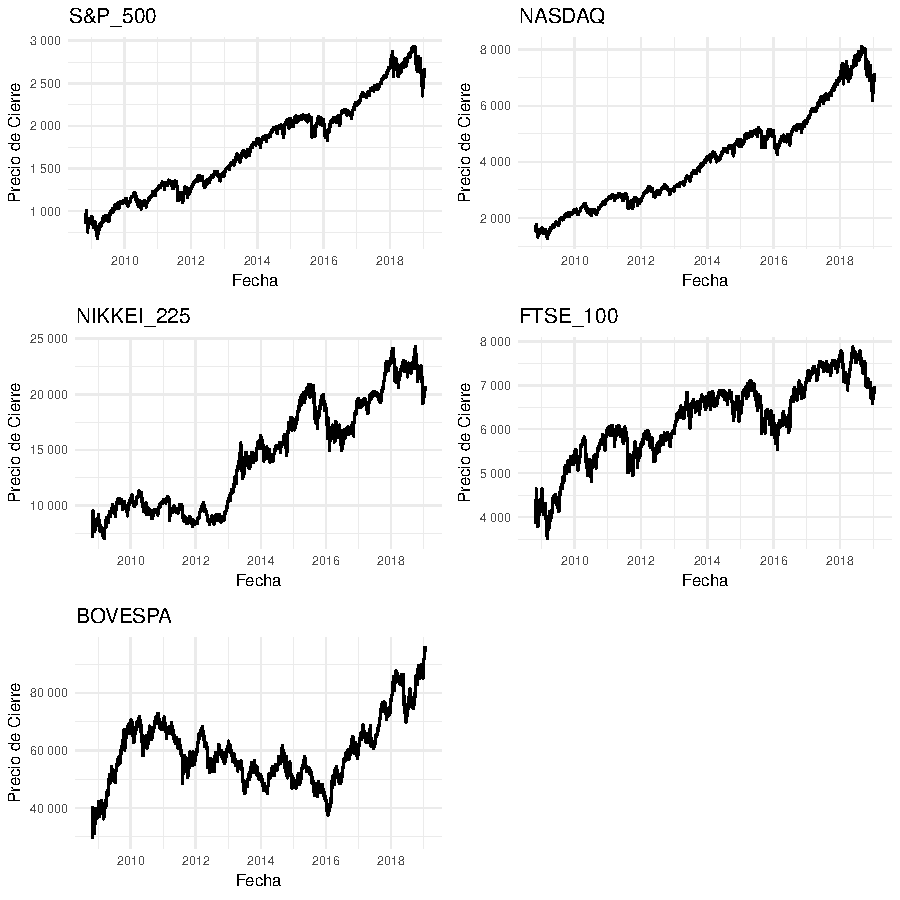
\includegraphics{main-002}
\caption{Precios de Cierre de los índices a utilizar en el período de estudio}
\end{figure}

\section{Entrenamiento del Modelo}

\subsection{Indicadores Técnicos como variables predictoras}

Los indicadores a utilizar fueron seleccionados buscando recoger la mayor información posible sobre el precio del activo que se pueden resumir en tres categorías: tendencia, momentum y volatilidad.

% <!-- Definir las 3 categorías -->

No es de interés en la presente investigación describir como funciona cada indicador para la toma de decisiones en el trading basado en fundamentos técnicos. Cada indicador puede utilizarse de distintas maneras, calcularse con distintos parámetros y asociarse a discreción del trader, lo que conlleva a un sin fin de reglas de asciación. 

Lo que busca la investigación es utilizar la relación entre estos indicadores como variables independientes que ayuden al modelo a predecir oportunidades de entradas. En este sentido se asume la existencia de una dinámica local del mercado que puede ser predecida con ayuda de estos indicadores.

\subsection{Variable dependiente}

Las decisiones de entrada en el trading pueden ser producto de muchos factores, en la presente investigación se analiza el enfoque donde se define un porcentaje objetivo de ganancia y se intenta predecir si dicho objetivo se materializará en un futuro cercano. Este enfoque reduce la toma de decisión en una variable tal que:

$$
P_{X}(x) = 
\begin{array}{ll} 
\ \ \ \ p \ ; \qquad x = c
\\
\ 1-p \ ; \qquad x = -d
\end{array}
$$

Dado los datos OHLC del activo es posible identificar los períodos en donde se materializa la variable dependiente, es decir, que el precio alcanza un porcentaje de ganancia sin antes haber retrocedido un porcentaje fijo. 

Se añade una columna con 'buy' para identificar los registros donde se da la señal y 'stay' en caso de que no haya ocurrido o hubiese ocurrido primero el retroceso del precio.

\subsection{Backtesting tipo WalkForward}

En principio se utilizó el método de entrenamiento, validación y prueba comúnmente utilizado, en donde la mayor parte de la data es destinada a entrenamiento del modelo, otra seccion es destinada a validación, para elegir los parámetros óptimos, y finalmente se testeaba el modelo en la data de prueba. Sin embargo este tipo de metodología en opinión del investigador no es el más óptimo dado el dinamísmo de los mercados bursátiles. 

Se opto por el metodo de backtesting Walkforward, el cual consiste en entrenar el modelo en un período base de data, en este caso los primeros 4 años de estudio, posteriormente se aplica la estrategia directamente en el año siguiente y se obtiene los primeros resultados. Luego este año de aplicación es incluído en la data de entrenamiento (es decir, la data de entrenamiento pasa a ser de 5 años) y se evalúa el modelo en el siguiente año. De esta manera, contemplamos el dinamismo del mercado permitiendole al modelo y por ende a la estrategia, utilizar el período mas reciente con respecto al cual será utilizada.

\begin{figure}[ht]
\begin{center}
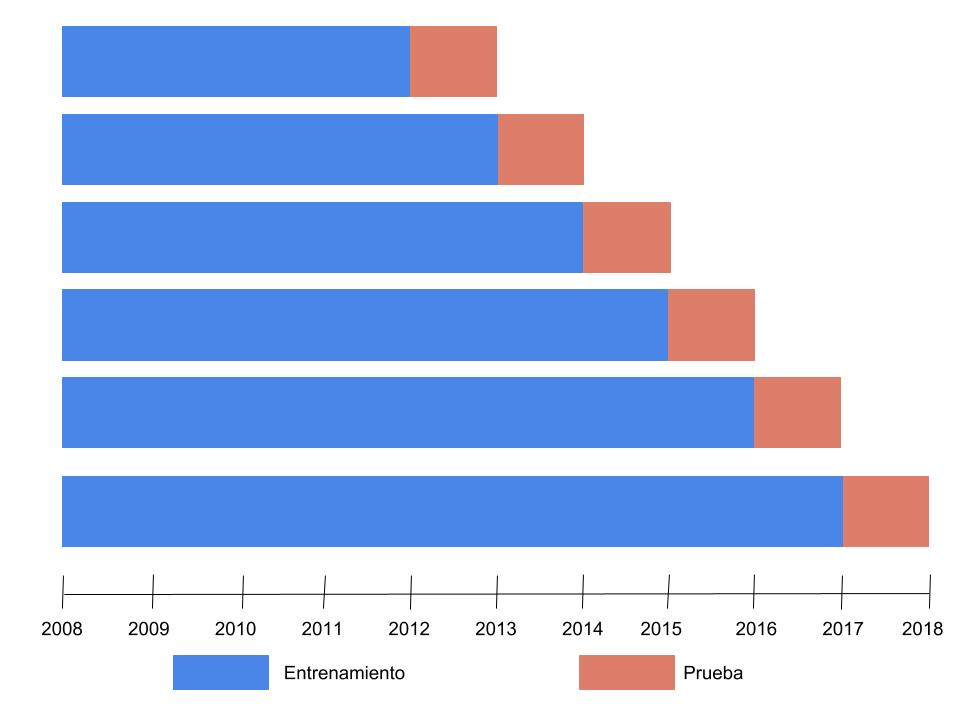
\includegraphics[width=2.5in]{images/walkforward_plot}
\end{center}
\caption{Metodología WalkForward}
\end{figure}

Otra de las caracteristicas de la metodología que se modificó fue la elección de los parámetros optimos. Previamente se utilizaba la data de validación para optimizarlos. Ahora bien en la metodología de Walkforward se utilizan los mismo dado la limitación en tiempo para programar una función que contemple todos las posibles configuraciones y elija la óptima. Sin embargo a opinión del investigador este enfoque también estaría limitado a un posible cesgo de sobreoptimización. El hecho de que en un año determinado unas configuraciones optimas den los mejores resultados no asegura que se replique en el siguiente año.

% Los datos son divididos en tres grupos: entrenamiento que representa 60\% del total de los datos, validación y prueba, cada uno representando 20\%. Los datos de entrenamiento son los que se utilizarán para enseñar al modelo a estimar la variable dependiente. Los datos de validación se utilizarán para definir la mejor combinación de parámetros (tp, sl y horizonte). Finalmente en los datos de prueba se aplica el modelo para obtener resultados simulando la estrategia.
% 
% En el estudio el 60\% de los datos de entrenamiento corresponden a los primeros 6 años (2009-2014) de muestra, la data de validación corresponde a los años (2015-2016) y la data de prueba los últimos dos años (2017-2018)

\subsection{Reducción de la dimensión con Análisis de Componentes Principales}

\subsection{Validación Cruzada en Series de Tiempo}

\subsection{Evaluación del desempeño del modelo}

En los problemas de clasificación se utiliza la matríz de confusión para evaluar el desempeño del modelo. La misma es una tabla que categoriza las predicciones realizadas por el modelo de acuerdo a la coincidencia con los valores reales. 

\begin{figure}[ht]
\begin{center}
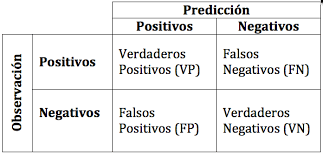
\includegraphics[width=2.5in]{images/confusion_matrix}
\end{center}
\caption{Matríz de Confusión}
\end{figure}

La estrategia solo toma la señal cuando el modelo predice un incremento en el precio, la venta por el contrario no depende del modelo, sino de los parámetros predefinidos. Esta característica condiciona al modelo a optimizar la prediccion de los verdaderos positivos, este indicador se conoce como $Precisión$.

$$ Precisión = \frac{VP}{VP + FN} $$

En principio se desconoce cuales debieran ser los parámetros (tp, sl y horizonte) con los que opere la estrategia. Para su estimación, se aplica el modelo entrenado en la data de validación y se obtiene la precisión del modelo para cada combinación de parámetros definidos previamente. 

% <!-- Grafica de seleccion de parametros e interpretar -->
% !TeX root = ./main.Rnw
%\SweaveUTF8

\chapter{Análisis de Resultados}

En el presente capítulo se realiza la descripción de los resultados obtenidos despues de la aplicación del método propuesto para el cálculo del VaR. De igual modo, se presentan los resultados arrojados por las pruebas de Backtesting realizadas a las estimaciones obtenidas y sus respectivos análisis.

\section{Series de Rendimientos}

A partir de las series de precios correspondientes a los commodities Petróleo, Oro, Cacao, Harina de Soja y  Aluminio; comprendidas entre el periodo $(10/2010 - 10/2018)$ se calcularon las series de rendimientos logaritmicos para cada uno de los activos. Cabe destacar que se disponen de 1679 observaciones de rendimientos diarios para cada commodity.





% !TeX root = ./main.Rnw
%\SweaveUTF8

\chapter*{Conclusiones y Recomendaciones}
\addcontentsline{toc}{chapter}{Conclusiones y Recomendaciones}

El estudio presentado se centró en confirmar alternativas eficaces para el cálculo del VaR en mercados de materias primas. Los hechos estilizados de las series de tiempo financieras fueron considerados a los largo del trabajo. Y frente a estos planteamientos, se desarrolló una investigación que permitiera detectar una aproximación con el método GARCH-EVT-COPULAS que tuviese la capacidad de estimar el riesgo del mercado de commodities.\\

% !TeX root = ./main.Rnw
%\SweaveUTF8

\chapter*{Lista de Referencias}
\addcontentsline{toc}{chapter}{Lista de Referencias}

\begin{itemize}

\item Alexander, N. Y Zafer, D. (2016). \textit{Gestión del riesgo con el uso de commodities energéticos utilizando Valor en riesgo y Teoría del Valor Extremo}. Suecia, Universidad de Lund.

\end{itemize}

\end{document}
